\documentclass{standalone}
\usepackage{pgfplots}
\pgfplotsset{compat=newest}

\begin{document}
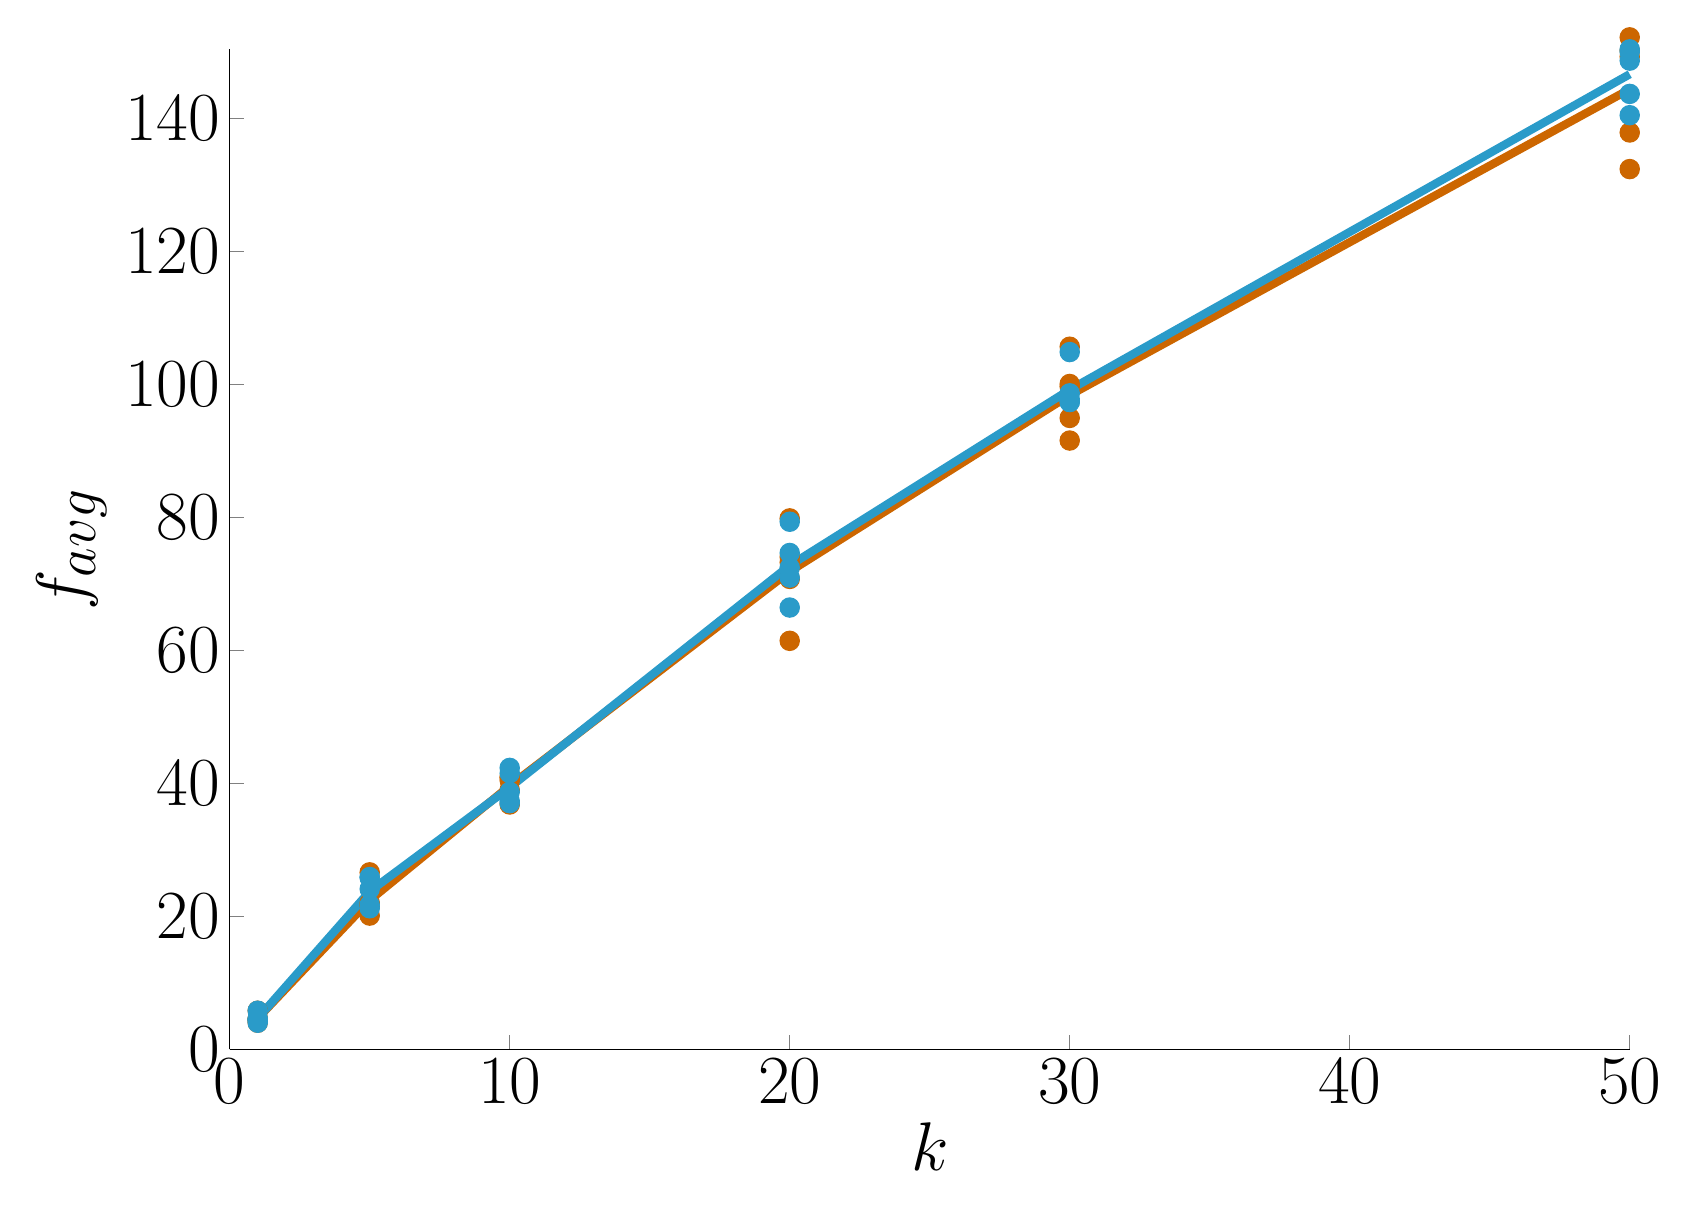
\begin{tikzpicture}

\begin{axis}[%
tick label style={font=\Huge},
label style={font=\Huge},
legend style={font=\Huge},
view={0}{90},
max space between ticks=50pt,
width=7in,
height=5in,
scale only axis,
xmin=0, xmax=50,
xtick={0, 10, 20, 30, 40, 50},
xlabel={$k$},
ymin=0, ymax=150.3,
%ytick={0, 200, 400, 600, 800, 1000},
ylabel={$f_{avg}$},
major tick length=5pt,
axis lines*=left,
legend cell align=left,
clip=false]

\addplot [
only marks,
mark=*,
mark size=3.5pt,
color=orange!80!black,
%solid,
%line width=2pt,
]
coordinates{
(1,4.0)(1,4.4)(1,4.5)(1,4.6)(1,5.8)(5,20.1)(5,21.6)(5,21.7)(5,22.0)(5,26.6)(10,36.8)(10,39.0)(10,40.4)(10,40.9)(10,40.9)(20,61.4)(20,70.7)(20,73.2)(20,74.0)(20,79.8)(30,91.5)(30,94.9)(30,99.6)(30,100.0)(30,105.6)(50,132.3)(50,137.8)(50,149.2)(50,150.1)(50,152.1)
};

\addplot [
only marks,
mark=*,
mark size=3.5pt,
color=cyan!80!black,
%solid,
%line width=2pt,
]
coordinates{
(1,4.0)(1,4.4)(1,4.5)(1,4.6)(1,5.8)(5,21.2)(5,21.7)(5,24.1)(5,25.8)(5,25.9)(10,37.0)(10,37.3)(10,38.7)(10,41.5)(10,42.3)(20,66.4)(20,70.9)(20,72.4)(20,74.6)(20,79.3)(30,97.3)(30,97.3)(30,97.7)(30,98.6)(30,104.8)(50,140.4)(50,143.6)(50,148.6)(50,149.9)(50,150.3)
};

\addplot [
color=orange!80!black,
solid,
line width=3pt
]
coordinates{
(1,4.66)(5,22.4)(10,39.6)(20,71.82)(30,98.32)(50,144.3)
};

\addplot [
color=cyan!80!black,
solid,
line width=3pt
]
coordinates{
(1,4.66)(5,23.74)(10,39.36)(20,72.72)(30,99.14)(50,146.56)
};


\end{axis}
\end{tikzpicture}
\end{document}
